\documentclass[9pt,journal,compsoc]{IEEEtran}
\ifCLASSOPTIONcompsoc
  \usepackage[nocompress]{cite}
\else
  \usepackage{cite}
\fi
\ifCLASSINFOpdf
\else
\fi
\hyphenation{op-tical net-works semi-conduc-tor}
\usepackage{cite}
\usepackage{amsmath,amssymb,amsfonts}
\usepackage{algorithmic}
\usepackage{graphicx}
\usepackage{textcomp}
\usepackage{xcolor}
\usepackage{graphicx}
\usepackage{subfigure}
\usepackage{CJK}
\usepackage{indentfirst}
\usepackage{amsmath}
\usepackage{upgreek}
\usepackage{tabu}
\usepackage{booktabs}
\usepackage{threeparttable}
\usepackage{tabularx}
\usepackage{multirow}
\usepackage{multicol}
\usepackage{arydshln}
\usepackage{makecell}


\begin{document}

\title{A High-Performance Design of Generalized Pipeline Cellular Array}

\author{
        Zhufei~Chu,~\IEEEmembership{Member,~IEEE,}
        Huiming~Tian,
        Zeqiang~Li,
        Yinshui~Xia,
        and Lunyao~Wang
        % <-this % stops a space
\thanks{
(\emph{Corresponding author}: \emph{Zhufei Chu}).
Z. Chu, H. Tian, Z. Li, Y. Xia, and L. Wang are with the Faculty of Electrical Engineering and Computer Science, Ningbo
University, Ningbo 315211, China. (email:chuzhufei@nbu.edu.cn)
}}

%\author{TBD}

%\author{Zhufei Chu,~\IEEEmembership{Member}, Huiming Tian, Lunyao Wang and Yinshui Xia\IEEEcompsocthanksitem J. Doe and J. Doe are with Anonymous University.s}
%       ~\IEEEmembership{}
%        ~\IEEEmembership{}
%\IEEEcompsocitemizethanks{\IEEEcompsocthanksitem M. Shell was with the Department
%of Electrical and Computer Engineering, Georgia Institute of Technology, Atlanta,
%GA, 30332.\protect\\
%E-mail: see http://www.michaelshell.org/contact.html
%\IEEEcompsocthanksitem J. Doe and J. Doe are with Anonymous University.}% <-this % stops an unwanted space
%\thanks{Manuscript received April 19, 2005; revised August 26, 2015.}}




\markboth{IEEE Computer Architecture Letters}%
{Chu \MakeLowercase{\textit{et al.}}: A High-Performance Design of Generalized Pipeline Cellular Array}

\IEEEtitleabstractindextext{%
\begin{abstract}
In this letter, we proposed a high-performance quantum-dot cellular automata (QCA) design of generalized pipeline cellular array (GPCA). The GPCA can perform all the basic arithmetic operations using only one arithmetic cell. Due to its flexibility, the high-performance GPCA design is of high interest for large-scale QCA designs.
We proposed both the arithmetic unit and control unit designs of GPCA using a hybrid logic network that represented by majority-of-three (MAJ), inverter (INV), and three-input exclusive-OR (XOR$_3$). The introduction of XOR$_3$ operation can significantly reduce the number of gates, levels, and inverters, which in turn results in less area and fewer clock cycles of QCA layout.  
On average, the proposed design can reduce the area and latency by 39.27\% and 35.89\% compared with the-state-of-art, respectively.
\end{abstract}

% Note that keywords are not normally used for peerreview papers.
\begin{IEEEkeywords}
majority, three-input XOR, pipeline cellular array, quantum-dot cellular automata (QCA)
\end{IEEEkeywords}}


% make the title area
\maketitle
\IEEEdisplaynontitleabstractindextext
\IEEEpeerreviewmaketitle
\IEEEraisesectionheading{\section{Introduction}\label{sec:introduction}}
\IEEEPARstart{C}{omplementary} metal-oxide-semiconductor (CMOS) technology is gradually reaching its physical limitation in recent years. Quantum-Dot Cellular Automata (QCA) is considered as one of the promising emerging nanotechnologies for its high speed, ultra-low power consumption and high density~\cite{1}. The principle for binary computing of QCA is based on Coulomb interactions. The polarization of electrons in a QCA cell can represent logic `0' and `1'. 

The primitives used in QCA are inverter (INV) and majority-of three (MAJ) gate which can be set to perform like AND/OR gates. 
The MAJ gate over three Boolean variables $a$, $b$, and $c$ can be represented as $\mathbb{M}(a,b,c)=ab+ac+bc$.
For the three-input XOR gate (XOR$_3$), it can be also represented as the MAJ forms, i.e., $\mathbb{X}(a,b,c)=a \oplus b \oplus c= \mathbb{M}(\bar a, \mathbb{M}(a,b,\bar c), \mathbb{M}(a,\bar b, c))$. By setting any one of the three inputs to constant, we can obtain AND/OR/XOR operations over the remaining non-constant inputs.
As an example, $ab=\mathbb{M}(a,b,0)$ and $a\oplus b = \mathbb{X}(a,b,0)$. Compared with the direct realization by the MAJ forms, an independent XOR$_{3}$ QCA gate with less area is proposed in~\cite{3} recently, which provides a fundamental block for MAJ/INV/XOR$_3$ based QCA designs.

Computer arithmetic plays a key role in modern computing. 
The implementations of various arithmetic circuits in QCA have been investigated in the literature, such as divider~\cite{sasamal2016design}, multiplier~\cite{lu2011qca,liu2013design}, squarer~\cite{giannou2012squarers}, and square rooting circuit~\cite{jahangir2015designing}, etc. 
Instead of specific arithmetic circuit design, a universal arithmetic unit named generalized pipeline cellular array (\textbf{GPCA}) which can perform all the basic arithmetic operations in pipeline manner was proposed in~\cite{4} and implemented in QCA by~\cite{2}. The GPCA consists of an adder-subtractor arithmetic unit (\textbf{AU}) and a control logic unit (\textbf{CU}). Unlike the work in~\cite{2} which focuses on realizing the GPCA only by MAJ and INV primitives, in this letter, we redesigned the AU and CU in GPCA using the combinations of MAJ, INV, and XOR$_3$ operations for high-performance design. The experimental results show that our design can averagely reduce the area and delay by 39.27\% and 35.89\%, respectively.
 
   
%A design of generalized pipeline cellular array (\textbf{GPCA}) which can perform all the basic arithmetic operations was proposed in~\cite{2}. However, it mainly focuses on realizing them only by MAJ and INV primitives. In this letter, we redesigned the AU and CU using the combinations of MAJ, INV, and XOR$_3$ operations. The experimental results show that our design can averagely reduce the area and delay by 39.27\% and 35.89\%, respectively.

\section{Proposed Designs}
In this section, we first review the Boolean logic networks by related work, then the proposed designs of the GPCA by using MAJ, INV, and XOR$_3$ primitives are presented.

\begin{figure}[t]
    \centering
    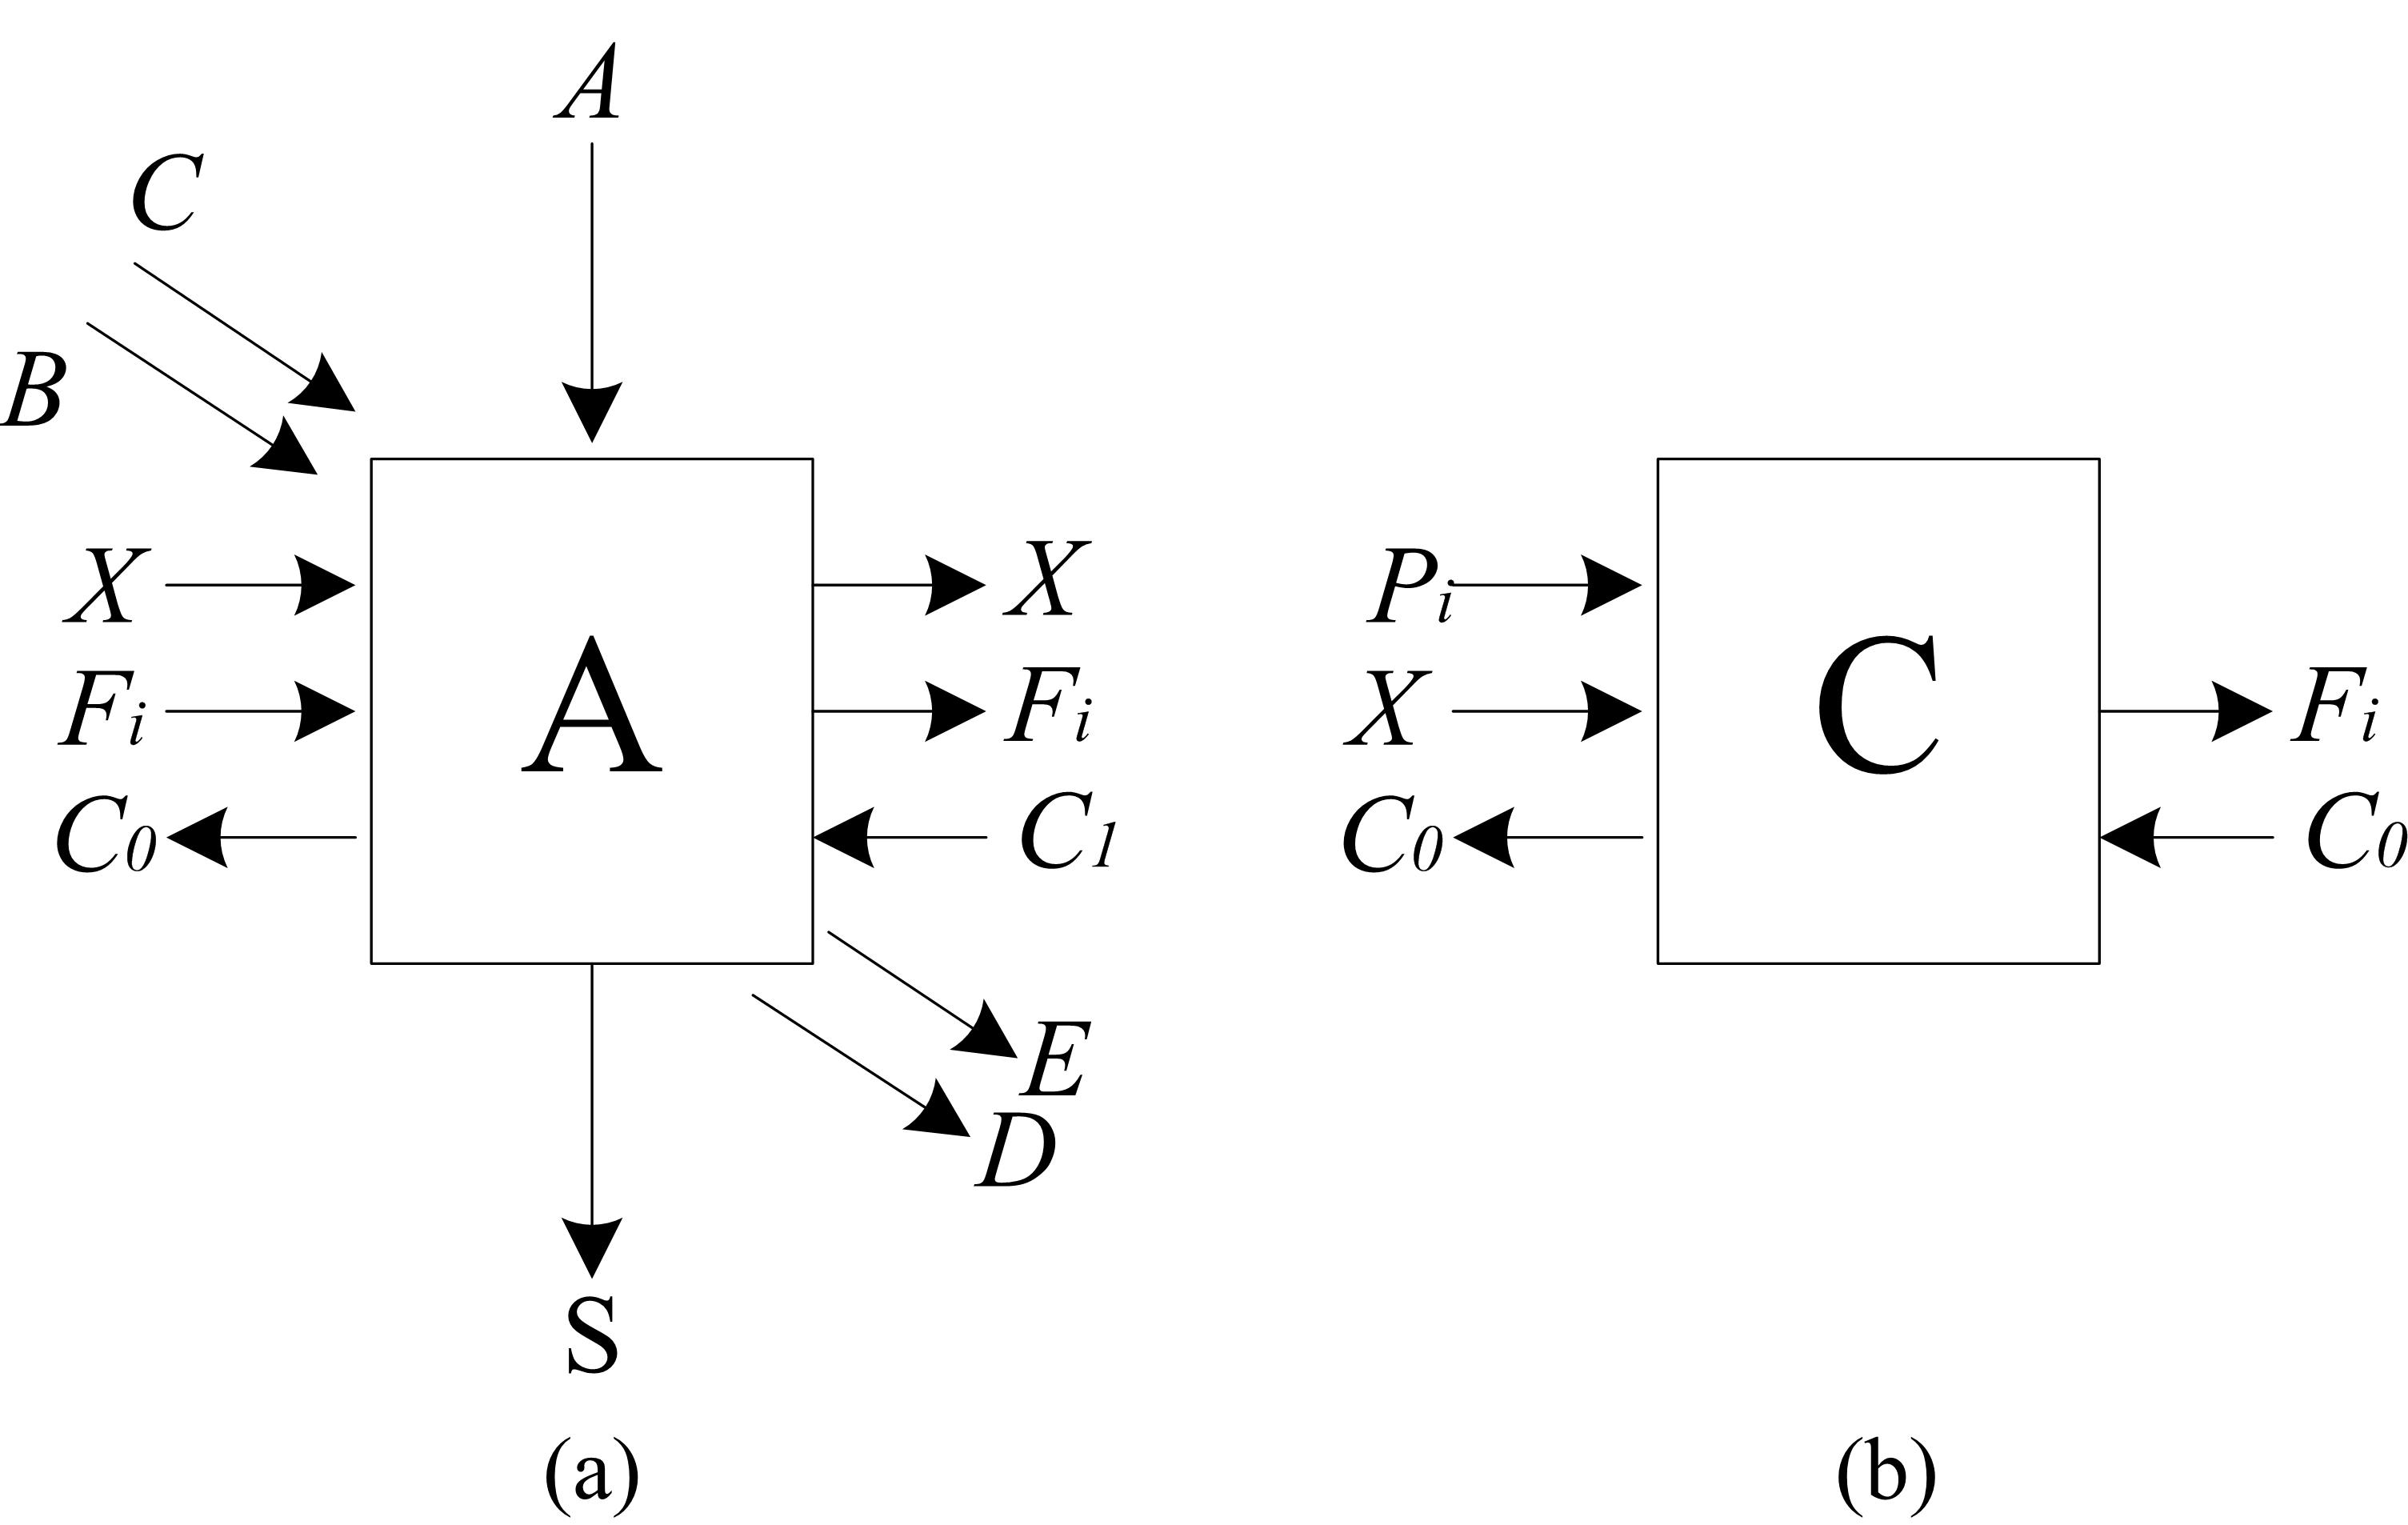
\includegraphics[width=2.0in]{fig/cell.jpg}
    \caption{Structure of the GPCA: (a) AU (b) CU} \label{fig:structure}
\end{figure}

\subsection{Boolean Expressions of the GPCA}
The GPCA contains AU and CU, the structures of which are shown in Fig.~\ref{fig:structure} (a) and (b), respectively.
The AU has six inputs, i.e., $A$, $B$, $C$, $F_{i}$, $X$, and $C_{1}$, and four outputs, i.e., $S$, $D$, $E$ and $C_{0}$.
The CU has three inputs, i.e., $C_{0}$, $P_{i}$, and $X$, and one output $F_{i}$.
The Boolean expressions of AU used in the work~\cite{4} are given as in~\eqref{eqs:au}.
\begin{equation}~\label{eqs:au}
\left.
\begin{split}
& S =(A \oplus (B \oplus X) \oplus C_{1}) F_{i} + A\overline{F_{i}} \\
&C_{0} = (B \oplus X)(A + C_{1}) + AC_{1} \\
&D =BC + CF_{i} = C (B + F_{i})\\    
&E =  B + CF_{i} = (B+C)(B+F_{i})\\
\end{split}\right\}
\end{equation}
For the CU part, the Boolean expression is defined by
\begin{equation}\label{eq:cu}
F_{i} = C_{0}X + P_{i}\bar{X}.
\end{equation}

Since QCA can natively implement MAJ and INV operations as the fundamental logic devices, the authors in~\cite{2} proposed a functional equivalent MAJ/INV based logic network. The Boolean expressions of AU are shown in~\eqref{eqs_maj:au}, where $n_0$, $n_1$, $n_2$, and $n_3$ are internal nodes.
\begin{equation}~\label{eqs_maj:au}
\left.
\begin{split}
& S = \mathbb{M}(\mathbb{M}(n_0, F_i, 0),\mathbb{M}(A, \bar F_i, 0 ), 1) \\
&C_{0} = n_1 \\
&D = \mathbb{M}(C, n_3, 0)\\    
&E = \mathbb{M}(B, C, n_3)\\
& n_0 = \mathbb{M}( \bar n_1, \mathbb{M}(n_2, \bar A, C_1), A )\\
& n_1 = \mathbb{M}(n_2, A, C_1) \\
& n_2 = \mathbb{M}(\mathbb{M}(\bar X, B, 0), \mathbb{M}(X, \bar B, 0 ), 1) \\
& n_3 = \mathbb{M}(B, F_i, 1)
\end{split}
\right\}
\end{equation}
The MAJ/INV based expression for the CU is defined by
\begin{equation}\label{eq:cu}
F_{i} = \mathbb{M}(\mathbb{M}(X, C_0, 0), \mathbb{M}(\bar X, P_i, 0 ), 1).
\end{equation}
In total, the logic network of AU proposed by~\cite{2} requires tweleve MAJ gates, six levels, and five INVs, while the CU needs three MAJ gates, two levels, and one inverter.

\subsection{MAJ/INV/XOR$_3$ based Designs}
We will explain the proposed Boolean expressions for all the output signals of AU first, then the design of CU will be presented.

In terms of the outputs $S$ and $C_0$, from~\eqref{eqs:au} we can see the
subexpression $(B \oplus X)$ is appeared in both expressions. Moreover, the internal node $n_2$ in~\eqref{eqs_maj:au} actually preforms the same operation using MAJ/INV primitives, i.e., $n_2 = B \oplus X$.
The recent exact synthesis approach~\cite{soeken2017exact} indicates the two- or three-input XOR functions can be realized by at least three MAJ gates. Hence, the expression of $n_2$ in~\eqref{eqs_maj:au} is already optimal in size and depth.
Since the XOR$_3$ gate was proposed in the literature, we make use of MAJ/INV/XOR$_3$ based expressions for the design.
For the output $C_0$, we replace $n_2$ as $\mathbb{X}(B, X, 0)$, then
\begin{equation}\label{ex_C0}
C_{0} = \mathbb{M}(\mathbb{X}(B, X, 0), A, C_{1})
\end{equation}

For the output $S$, since $(a \oplus b)c + a\bar c = a \oplus bc$ holds, we can assign $a = A$, $b = (B \oplus X) \oplus C_1$, and $c = F_i$. Then
the expression of $S$ in~\eqref{eqs:au} is rewriten as
\begin{subequations}\label{ex_S}
\begin{align}
S &= (((B \oplus X) \oplus C_1)F_i) \oplus A \notag \\
  &= \mathbb{X}(\mathbb{M}(\mathbb{X}(B, X, C_1), F_i, 0), A, 0) \label{eq:S1}\\
  &= \mathbb{X}(\mathbb{M}(\mathbb{X}(\mathbb{X}(B, X, 0), C_{1}, 0), F_{i}, 0), A, 0). \label{eq:S2}
\end{align}
\end{subequations}
Equation~\eqref{eq:S1} requires only three MAJ/XOR$_3$ operations, in contrast, equation~\eqref{eq:S2} needs one additional XOR$_3$ operation but it can share the node $\mathbb{X}(B, X, 0)$ appeared in~\eqref{ex_C0}.
We reserve both the designs for further evaluations in QCA technology.

\begin{figure}
\centering
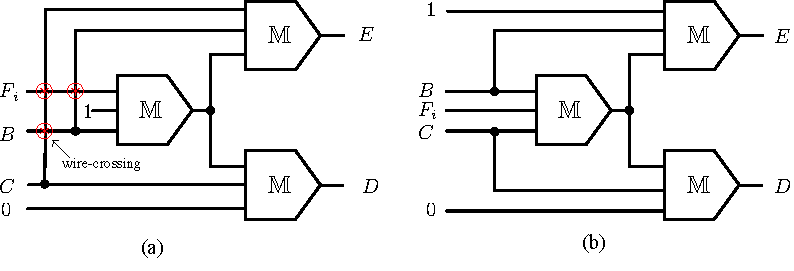
\includegraphics[width=3.5in]{fig/wire_cross.pdf}
\caption{Two logic networks for the outputs $D$ and $E$, (a) The expressions proposed by~\cite{2} may face wire-crossing problem, (b) Our design.}
\label{fig:wire_cross}
\end{figure}


The outputs of $D$ and $E$ is relatively simple. The logic network proposed by~\cite{2} is shown in Fig.~\ref{fig:wire_cross}(a), in which signals may face the wire-crossing problem. Minimizing the number of wire-crossing in the logic network is of high interest for the QCA technology~\cite{nath2017optimal}.
For the single-layer restriction, the wire-crossing cannot be implemented.
Moreover, too many wire-crossings increase the design complexities of a QCA layout since more area and timing are required.

The proposed logic network for outputs $D$ and $E$ is shown in Fig.~\ref{fig:wire_cross}(b), in which the wire-crossing problem is solved.
For the output $D$, the expression is
\begin{equation}\label{eq:D}
D = \mathbb{M}(\mathbb{M}(F_{i}, B, C), C, 0).
\end{equation}
By expansion and simplification, one can verify the function equivalence of~\eqref{eq:D} and the $D$ expression in~\eqref{eqs_maj:au}.
\begin{equation}
\begin{split}
D &= (F_iB + F_iC + BC)C = F_iBC + F_iC + BC \\
  &= F_iC + BC = (F_i + B)C \\
  &= \mathbb{M}(\mathbb{M}(F_i, B, 1), C, 0 )
\end{split}
\end{equation}
Similarly, the output $E$ is represented as
\begin{equation}\label{eq:E}
E = \mathbb{M}(\mathbb{M}(F_{i}, B, C), B, 1)
\end{equation}
such that the subexpression $\mathbb{M}(F_{i}, B, C)$ is shared with~\eqref{eq:D}.

\begin{figure}[t]
\centering
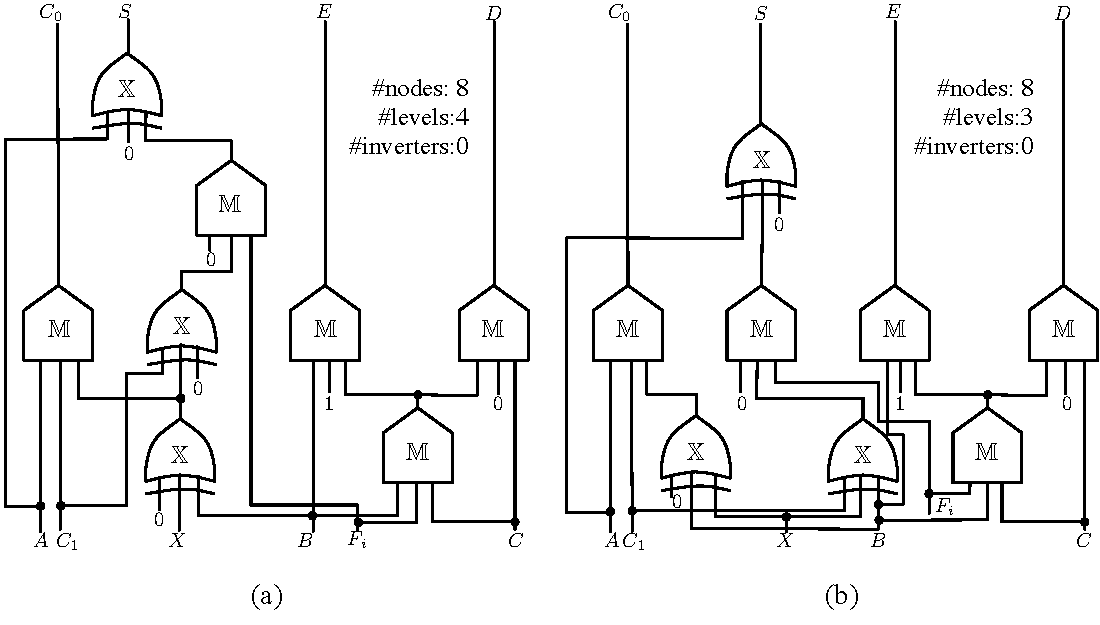
\includegraphics[width=3.5in]{fig/au_netlist.pdf}
\caption{The logic networks of the proposed design of AU, we make use of (a) \eqref{eq:S2}, (b)~\eqref{eq:S1} as the expression for the output $S$.}
\label{fig:au_netlist}
\end{figure}

 \begin{figure}[b]
     \centering
     \subfigure[]{
             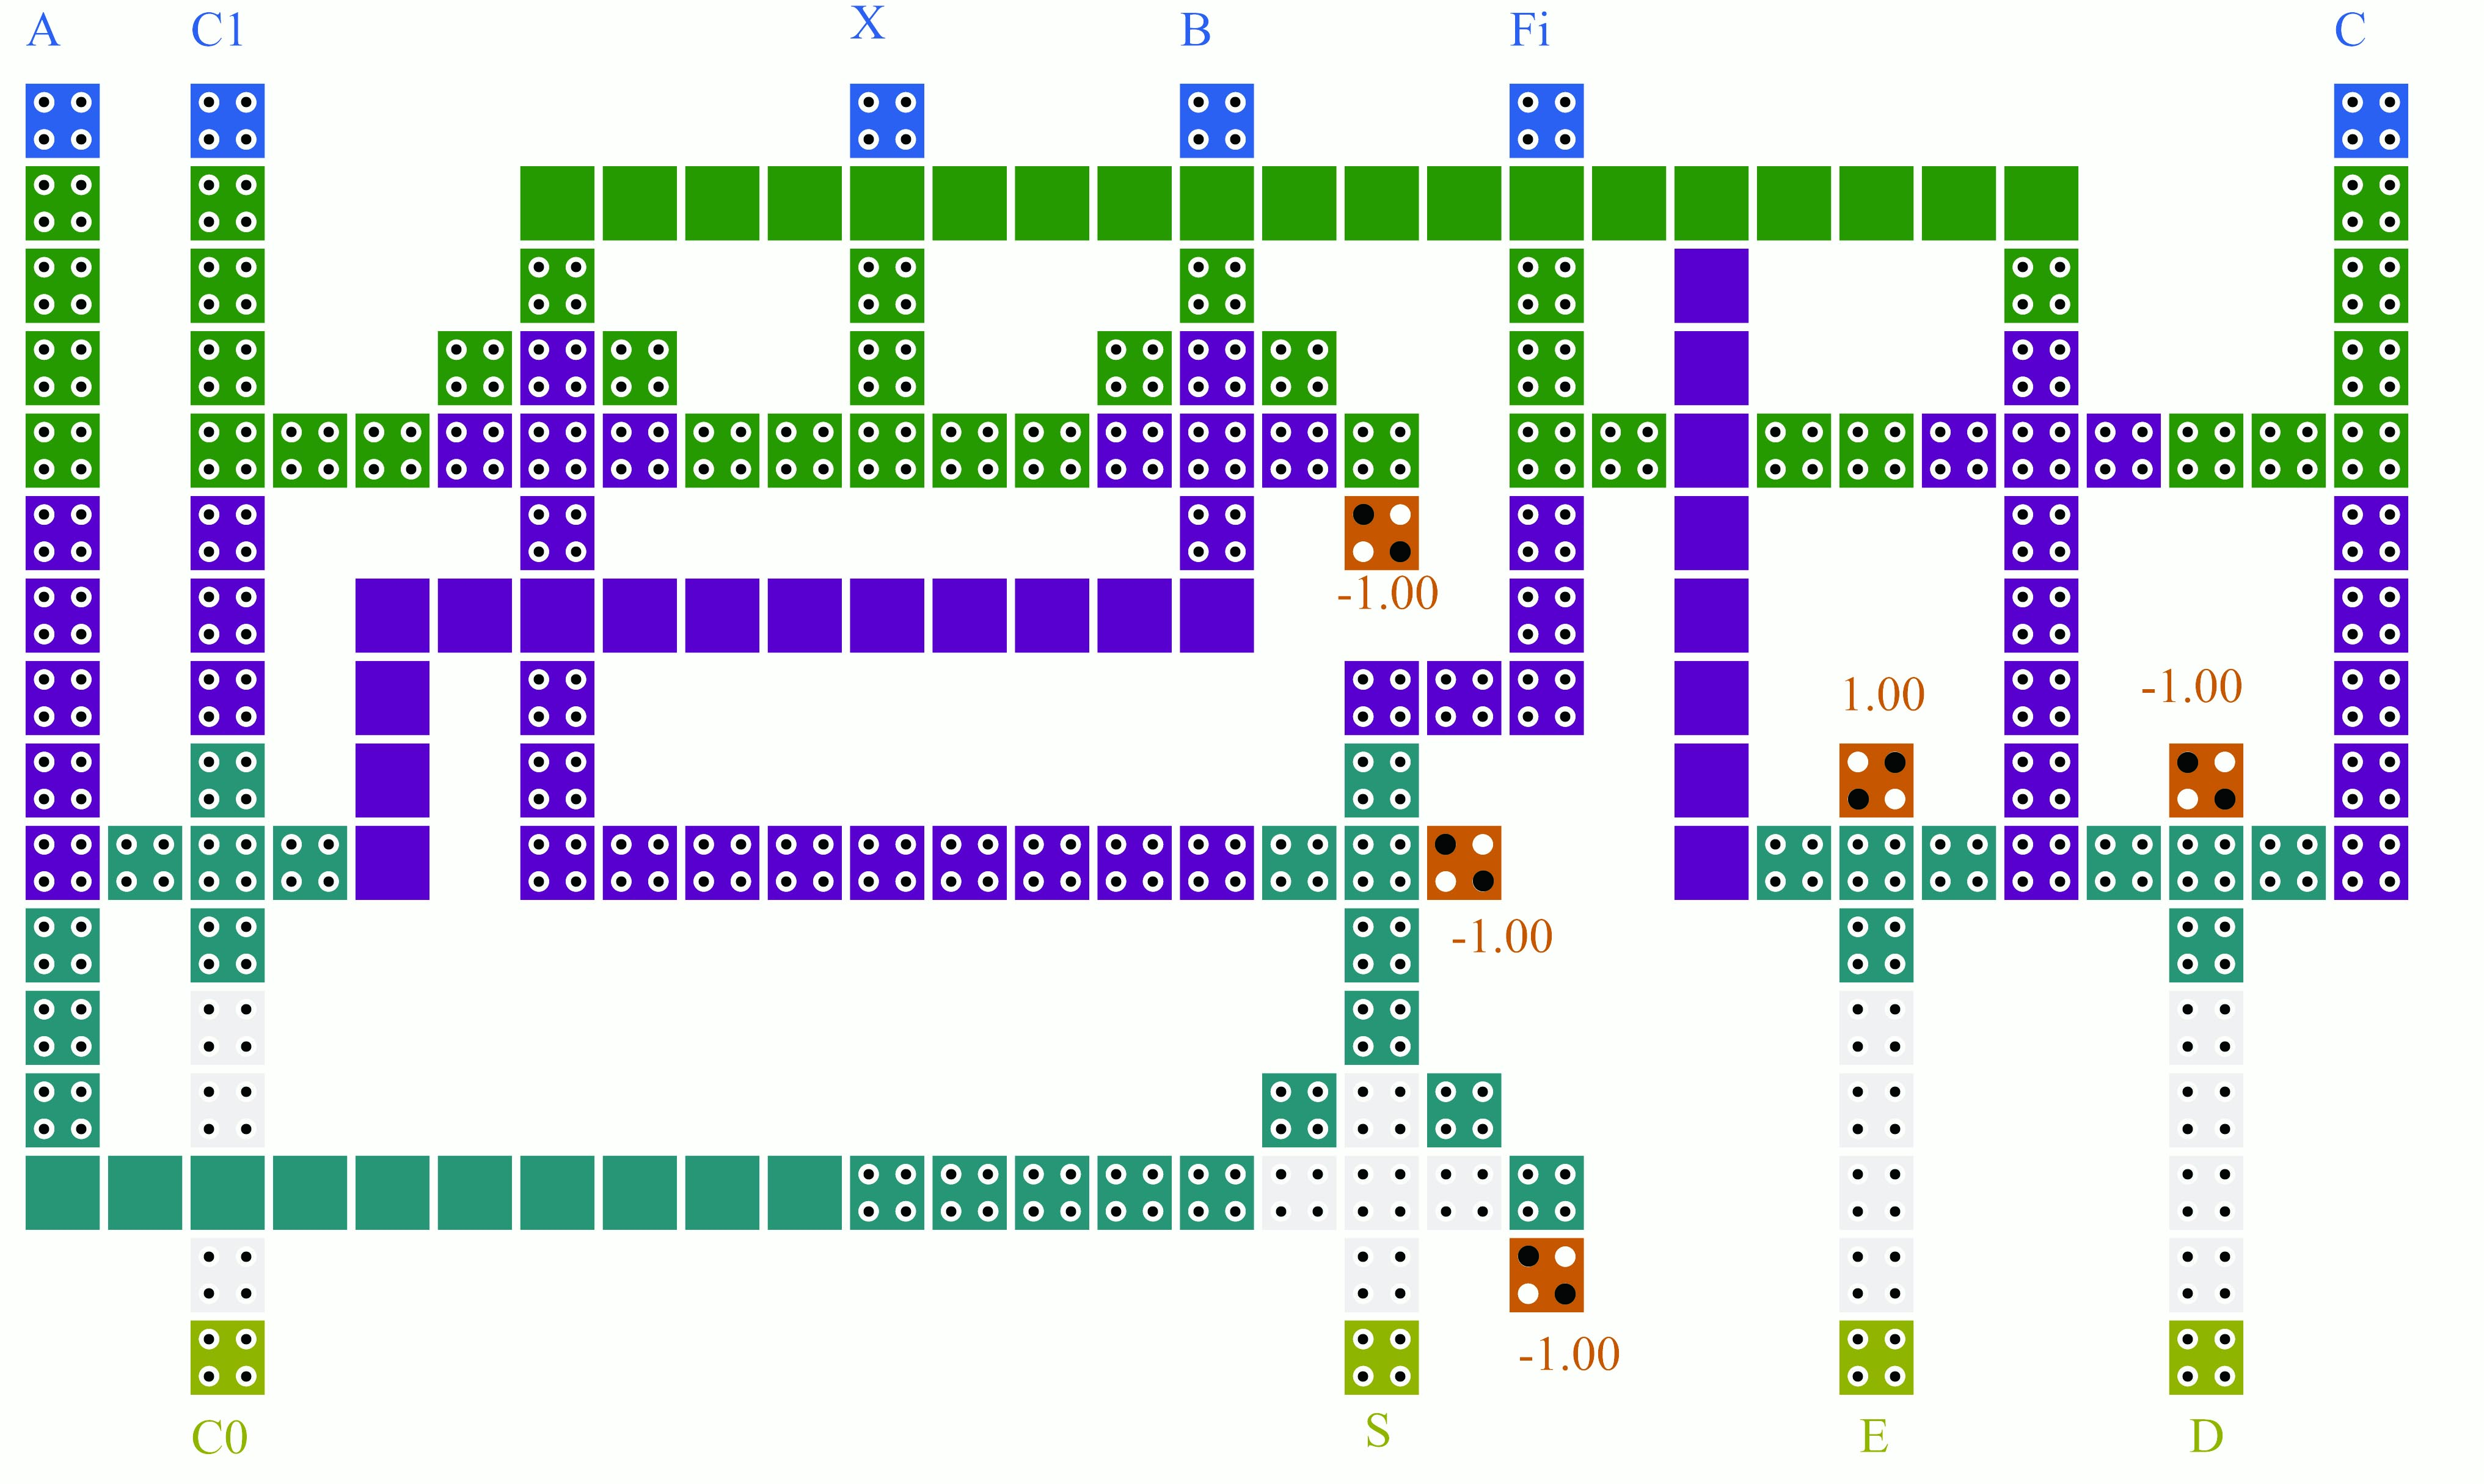
\includegraphics[width=2in]{fig/AU_xor3.jpg}
     }
     \subfigure[]{
            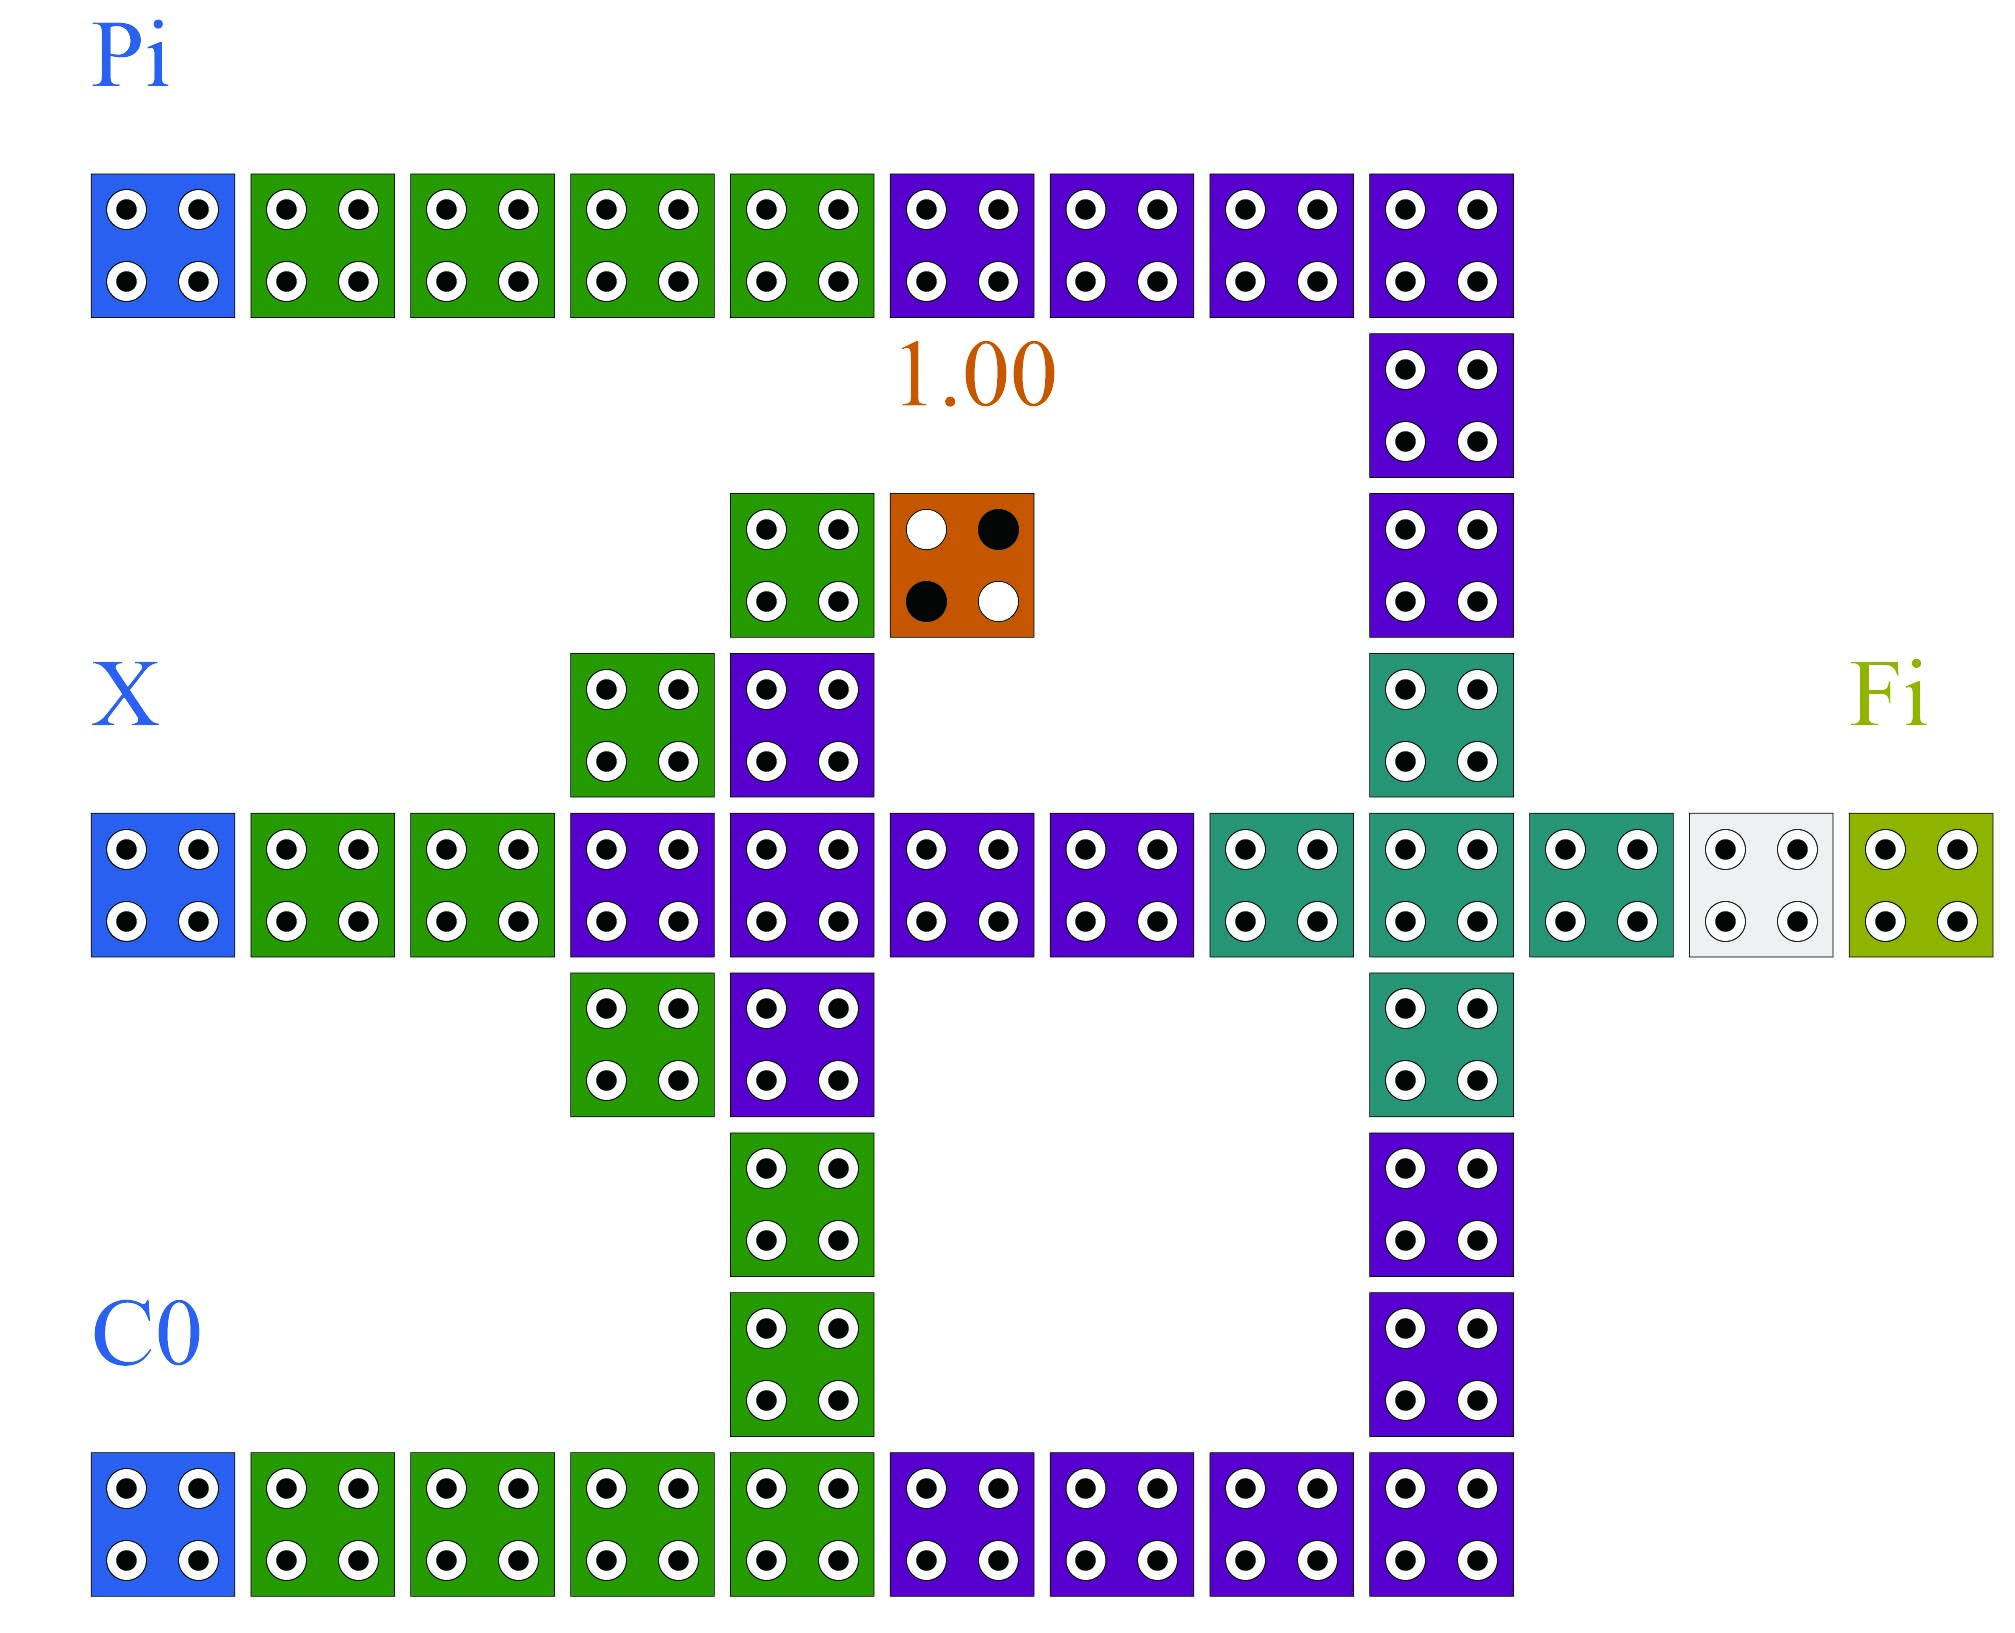
\includegraphics[width=0.8in]{fig/control_cell.jpg}
     }
     \caption{The QCA layout of the proposed designs (a) AU (b) CU}\label{fig:cu_au}
 \end{figure}

The expressions of the AU are the collections of equations~\eqref{ex_C0},~\eqref{ex_S},~\eqref{eq:D}, and~\eqref{eq:E}.
Since~\eqref{ex_S} has two versions of expression, i.e., \eqref{eq:S1} and \eqref{eq:S2}, we present the logic network of both of the two versions in Fig.~\ref{fig:au_netlist}.
Both of the designs require eight gates, including five MAJ gates and three XOR$_3$ gates. The number of logic levels of Fig.~\ref{fig:au_netlist}(b) is three while the one in Fig.~\ref{fig:au_netlist}(a) is four.
Besides, no inverters are required for both of the designs.
The main difference is the usage of the XOR$_3$ operation. Fig.~\ref{fig:au_netlist}(b) contains one fully-utilized XOR$_3$ node by rewriting $(B \oplus X) \oplus C_1$
into $\mathbb{X}(B, X, C_1)$. Since the node $\mathbb{X}(B, X, 0)$ has two fanouts in Fig.~\ref{fig:au_netlist}(a), we still need this node in~Fig.~\ref{fig:au_netlist}(b) for functional equivalence.
In comparison, the design proposed in~\cite{2} requires twelve MAJ gates, six levels, and five inverters. Thus, our design has more compact representations.

\begin{figure*}[t]
    \centering
    \includegraphics[height=12cm]{fig/pipeline_array.jpg}
    \caption{ The QCA layout of our proposed array}
\end{figure*}
%%%%%%%%%%%%%%%%%%%%%%%%%%%%%%%%%%%%%%%%%%%%%%%%%%%%%%%%%%%%%%%%%%%%%%%
\begin{table*}[h]
\caption{Comparisons of the proposed GPCA and the designs in~\cite{2}}
\centering
\begin{tabularx}{\textwidth}{Xrrrrrrrrr}
\toprule
            \multirow{2}{*}{Designs}& \multicolumn{3}{c}{\cite{2}}&\multicolumn{6}{c}{ Proposed }\\
            \cmidrule(lr){2-4} \cmidrule(lr){5-10}
            &Area ($\mu m^2$) & Latency & Cells count &Area ($\mu m^2$) & \% &Latency & \% & Cells count &\% \\
            \midrule
            Arithmetic cell &0.68 &4 &682 &0.21 &69.12 &1 &75 &217 &68.18 \\
            Control cell & 0.11&1.5&77&0.05&54.55&1&33.33&44&42.86\\
            Pipeline Array(n=3)&23.35&34&15098&17.06&26.94&25&26.47&10312&31.70\\
            Pipeline Array(n=4)&39.44&51&26698&29.80&24.44&39&23.53&17258&35.36\\
            Pipeline Array(n=5)&59.47&71&42174&46.80&21.30&56&21.13&26094&38.13\\
            \midrule
            Average improvement&  &  & & & 39.27\% & &35.89\% && 43.25\% \\
            \bottomrule
\end{tabularx}~\label{tab:result}
\end{table*}
%%%%%%%%%%%%%%%%%%%%%%%%%%%%%%%%%%%%%%%%%%%%%%%%%%%%%%%%%%%%%%%%%%%%%%%


\begin{figure*}[h]
    \centering
    \subfigure[]{
        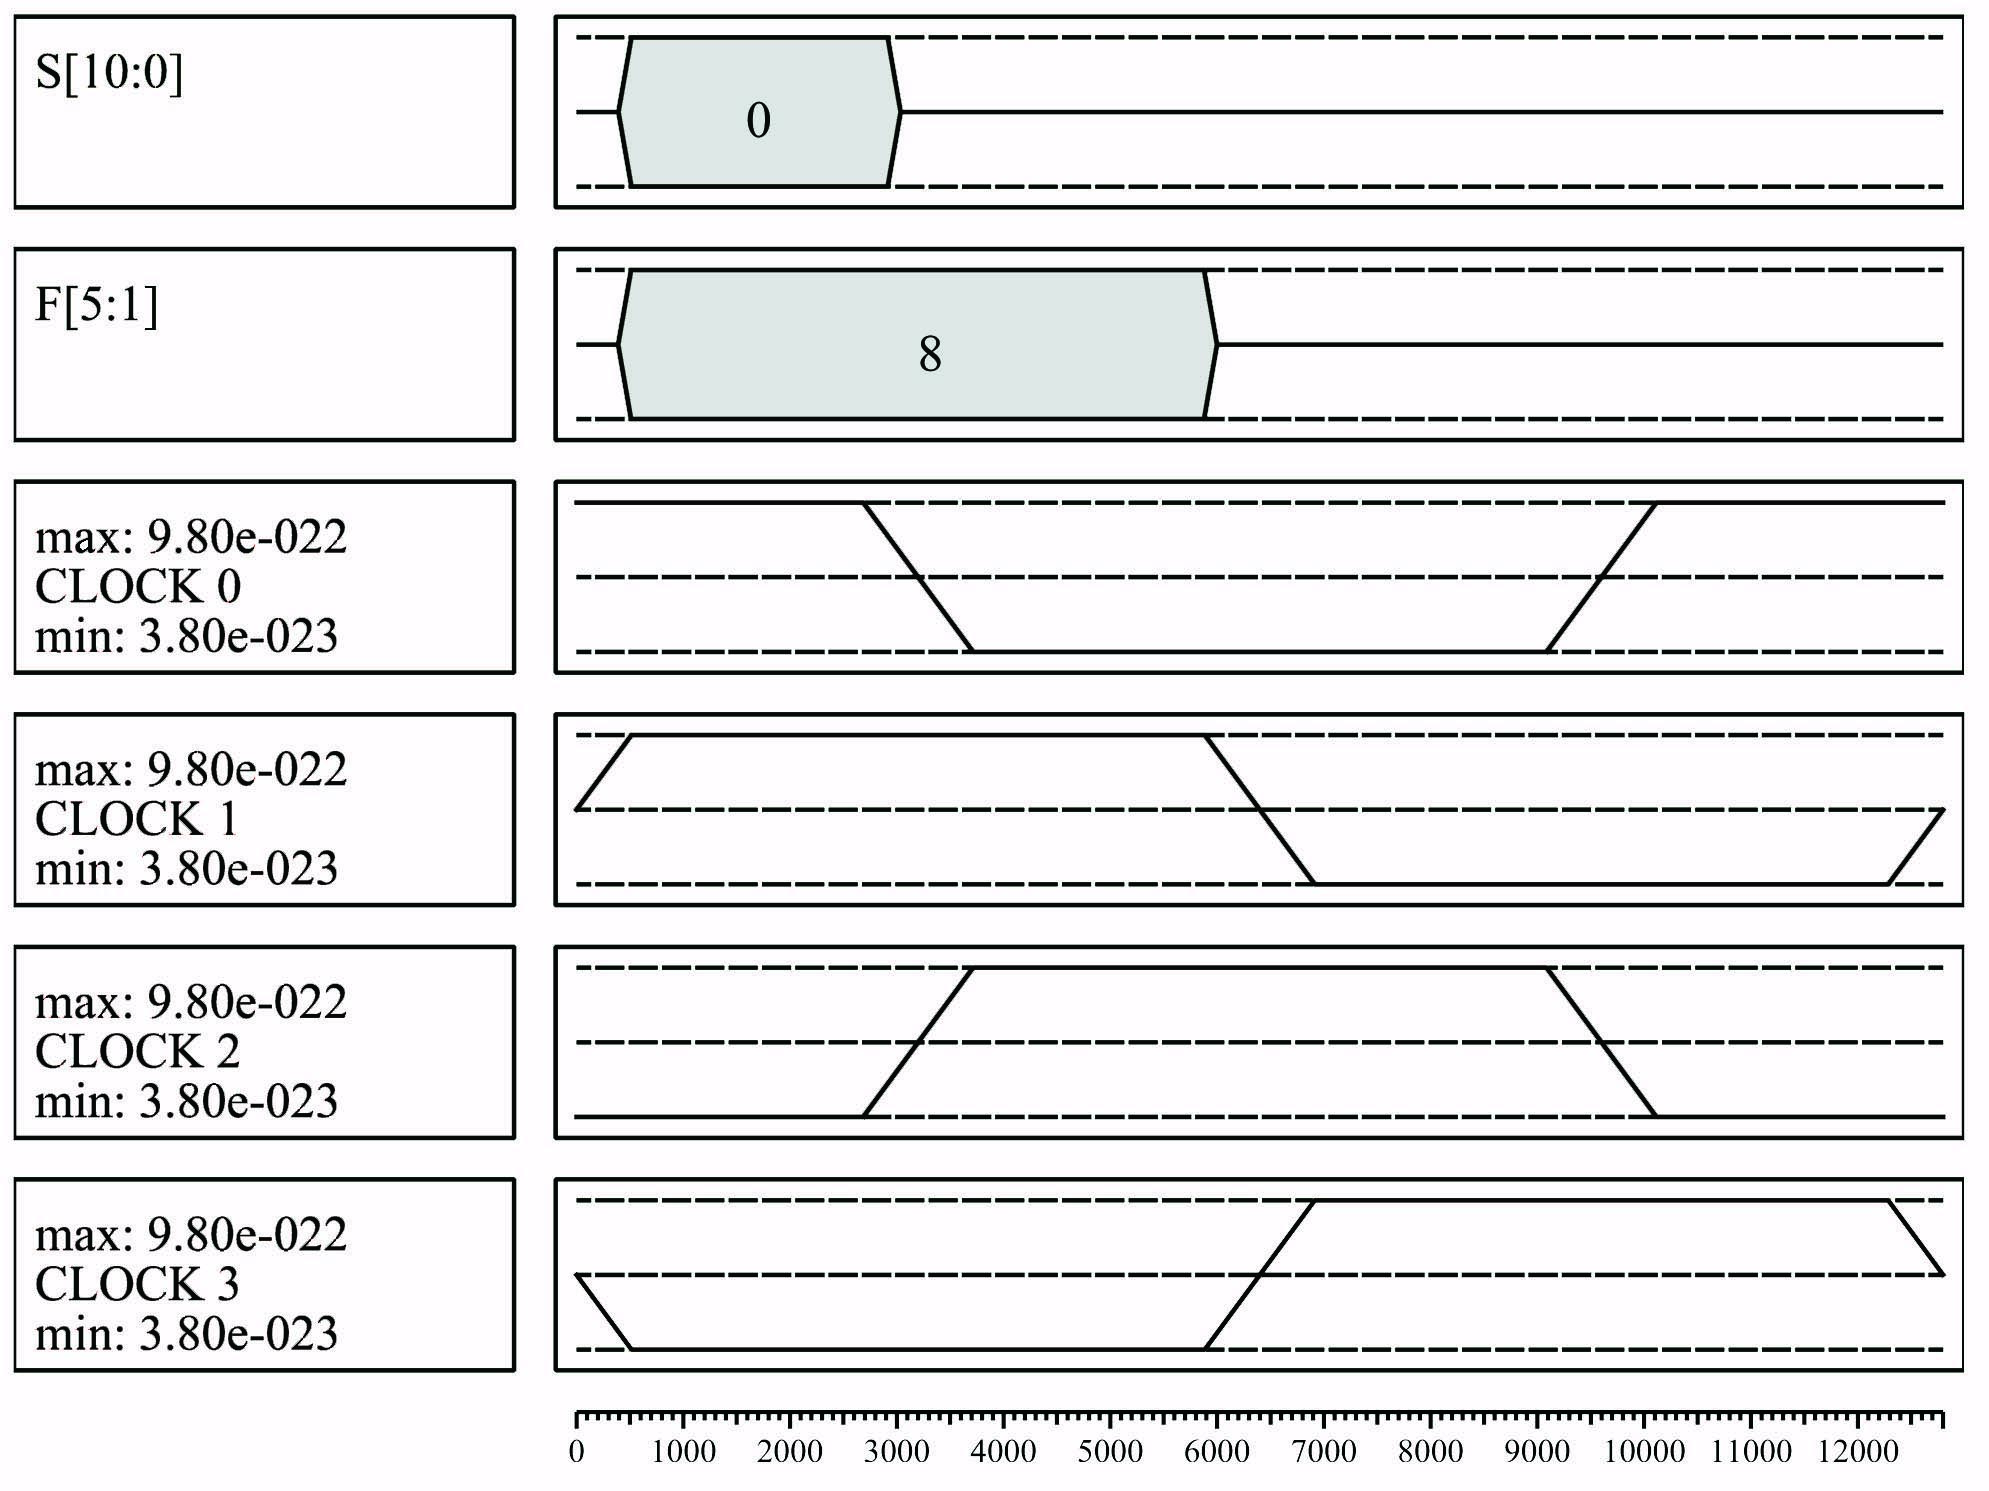
\includegraphics[width=1.65in]{fig/div.jpg}\label{div}
    }
    \subfigure[]{
        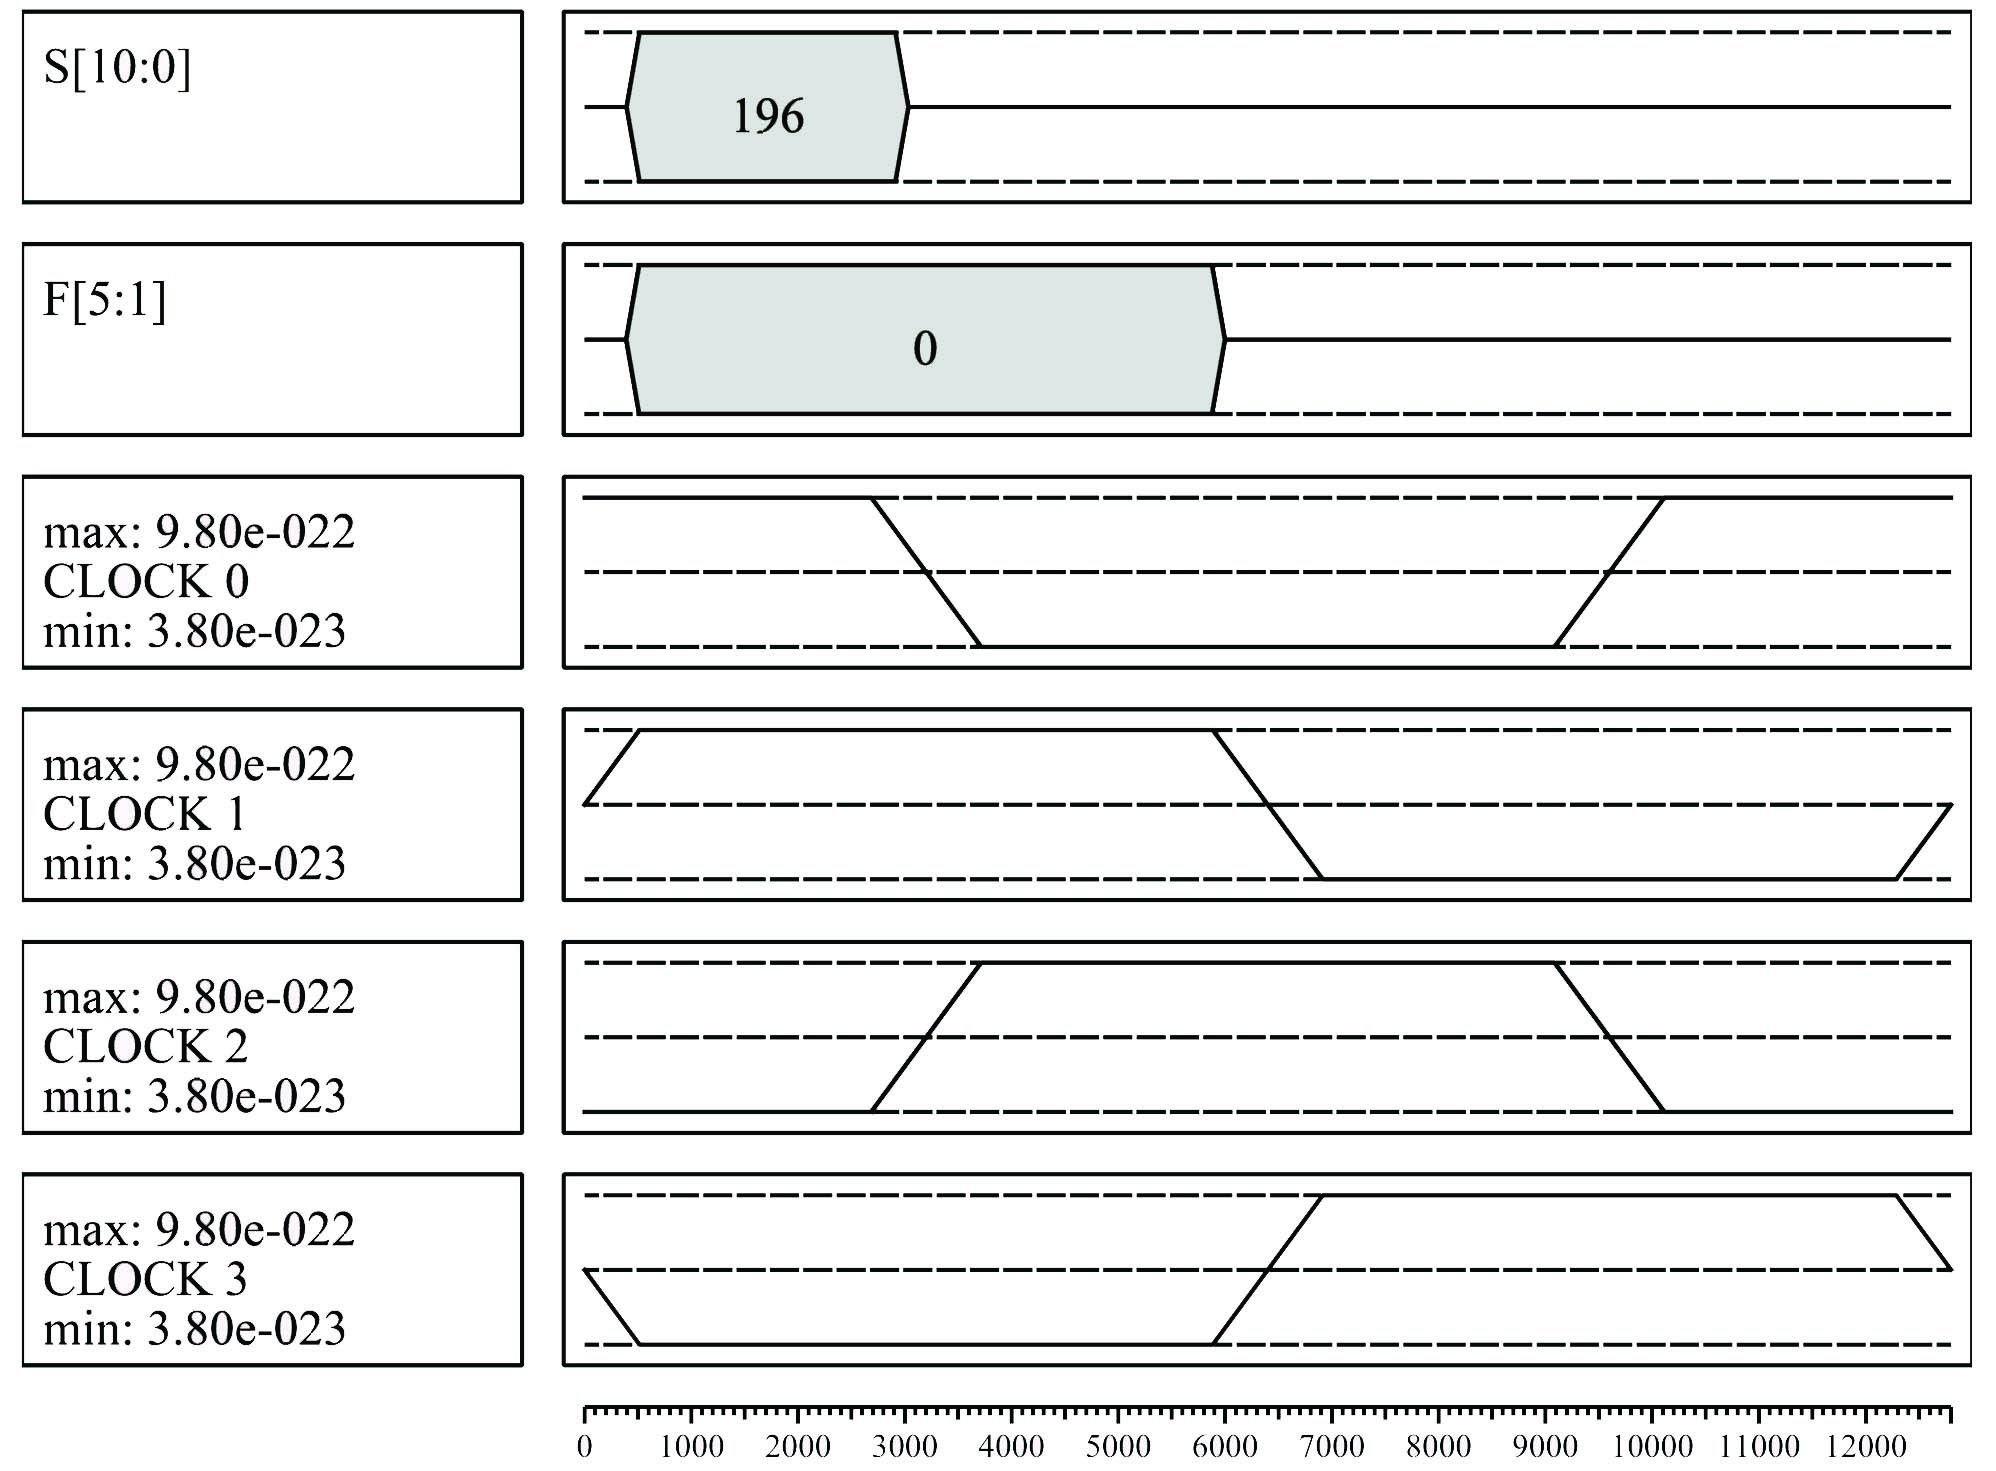
\includegraphics[width=1.65in]{fig/square.jpg}\label{square}
    }
    \subfigure[]{
            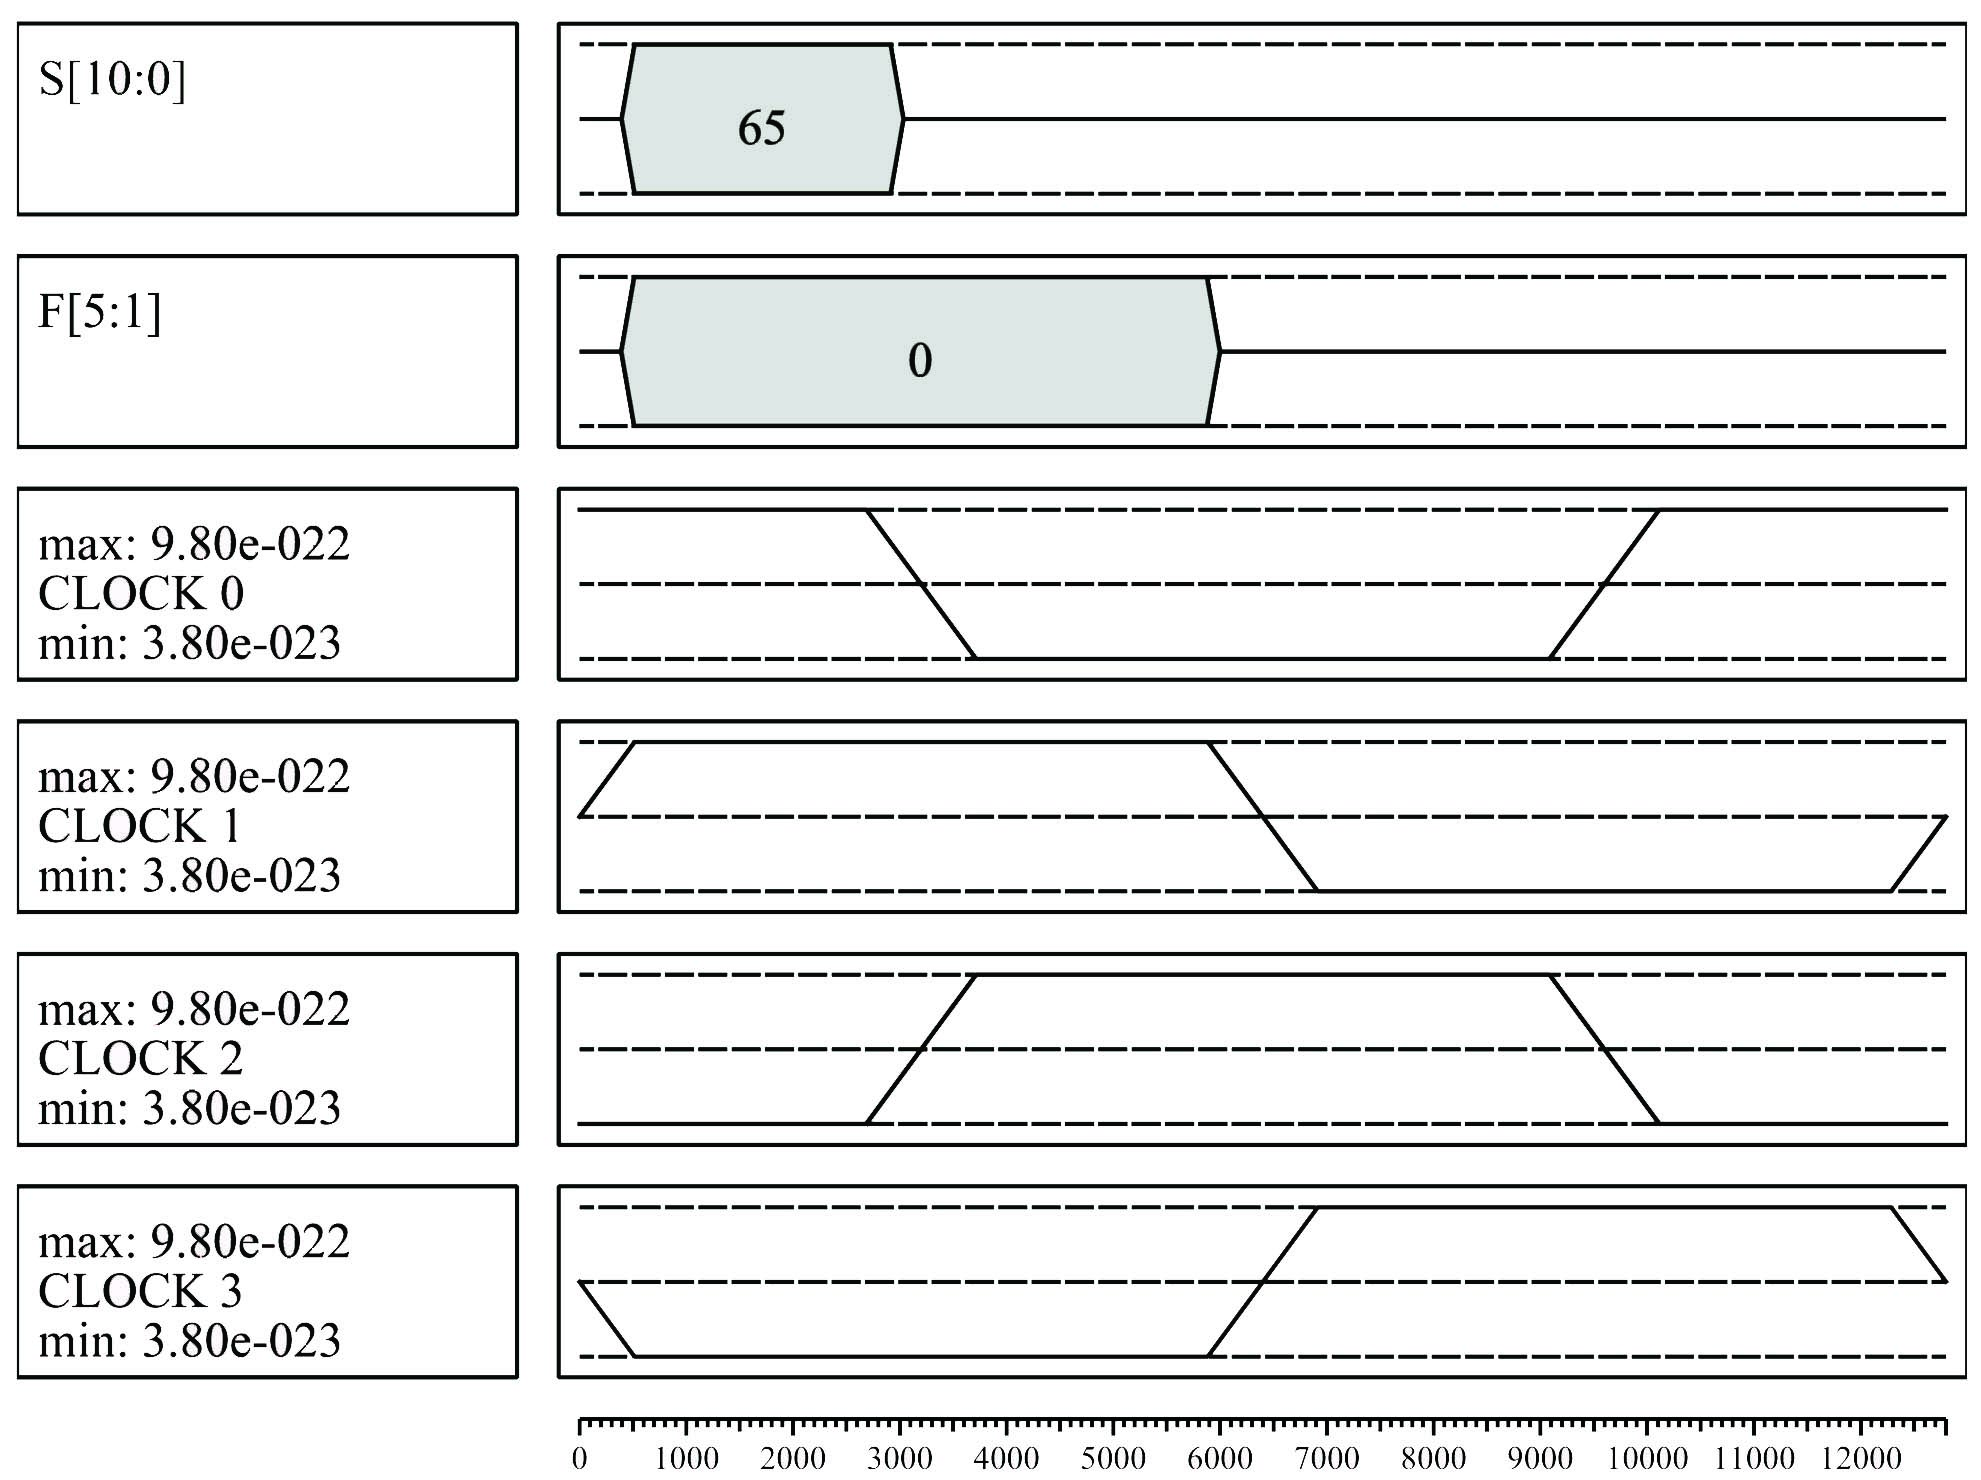
\includegraphics[width=1.65in]{fig/multiplier.jpg}\label{multiplier}
    }
    \subfigure[]{
          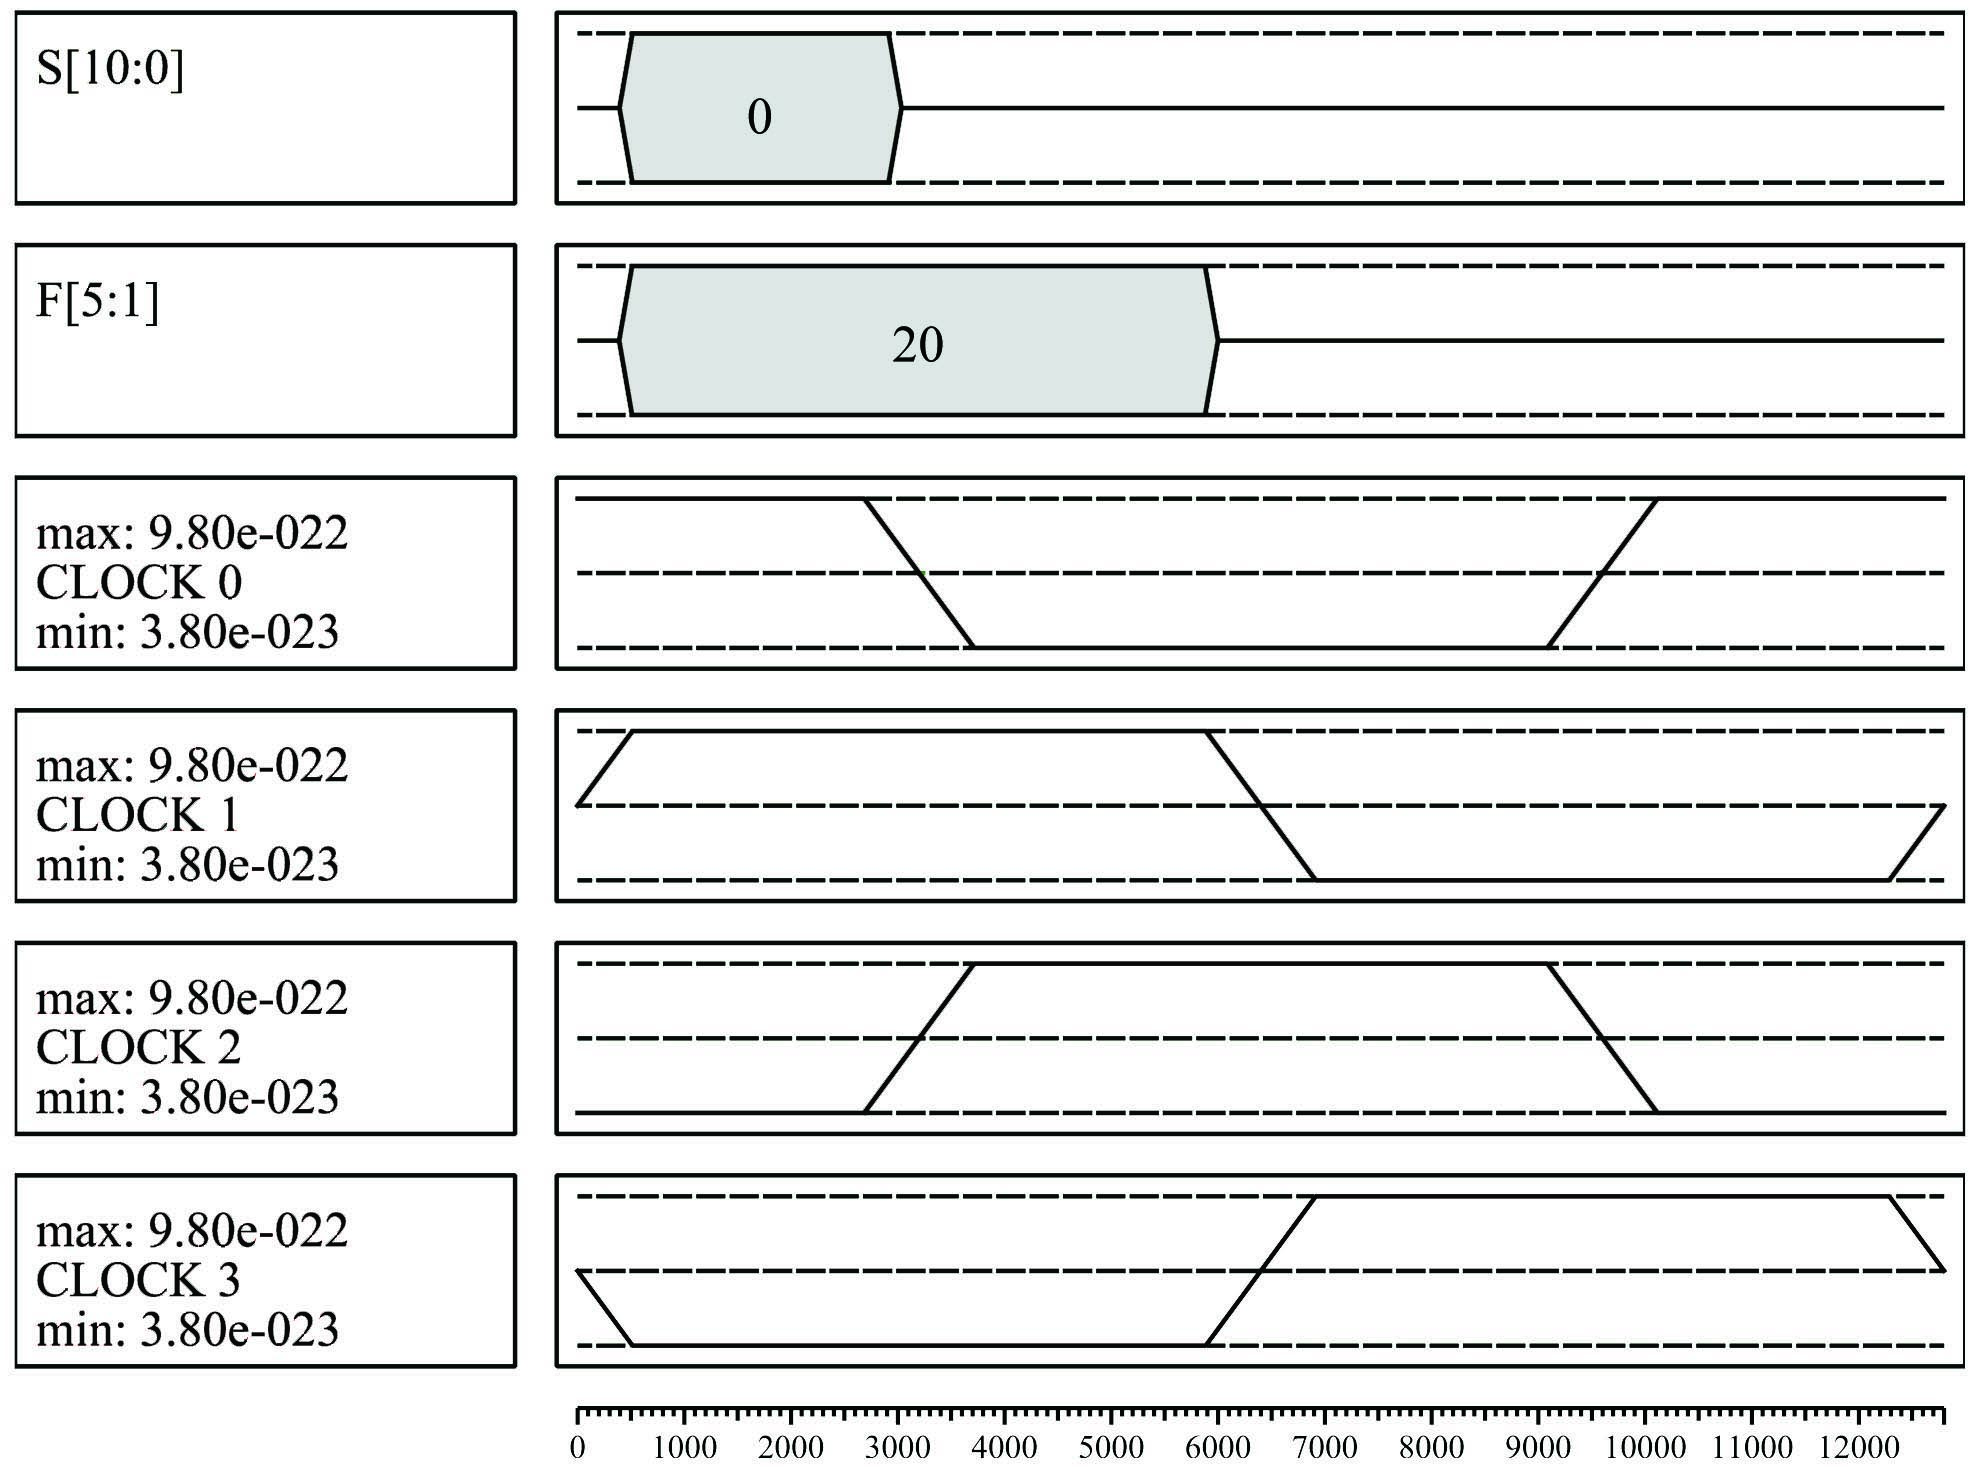
\includegraphics[width=1.65in]{fig/square_rooting.jpg}\label{square_rooting}
    }
    \caption{Simulation results for (a) Division of 10000 by 10 (b)Squaring of 1110 (c) Multiplication of 1101 and 101 (d)Square rooting of 110010000 }\label{tt_array}
\end{figure*}



In terms of CU part, the design proposed in~\cite{2} needs three MAJ gates and one inverter. Due to $ab + \bar b c = \mathbb{M}(a, c, \overline{a \oplus b}) = \mathbb{M}(a, c, \mathbb{X}(a,b,1))$, we can assign $a = C_0$, $b = X$, and $c = P_i$. Then the expression of $F_i$ can be rewritten as
\begin{equation}\label{Fi_xmg}
F_{i} = \mathbb{M}(\mathbb{X}(X,C_{0},1),P_{i},C_{0}).
\end{equation}
Note that a constant `1' input in XOR$_3$ gate leads to the inversion of the XOR operation over the other two inputs. Hence, the inverter is also eliminated thanks to the usage of XOR$_3$ operation.

\begin{table}[t]
\caption{Comparisons of the proposed two AU designs}
    \centering
    \begin{tabularx}{\linewidth}{Xcccc}
            \hline
        Designs & Area ($\upmu m^{2}$)& Latency & Cells count & Logic levels \\
        \hline
        Fig.~\ref{fig:au_netlist}(a) & 0.25      & 1.5            & 238               & 4            \\
        Fig.~\ref{fig:au_netlist}(b) & 0.21      & 1              & 217               &3             \\
        \hline
        Improvement & 16\%   & 33.33\%        & 8.82\%           & 25\%      \\
        \hline
    \end{tabularx}
    \label{tab:au}
\end{table}

\section{Simulation Results and Comparison}
In this section, the simulation results of our designs were presented.
All the designs and simulations are done by QCADesigner 2.0.3~\cite{QCAdesigner}.
We have set the same parameters with the ones used in~\cite{2}, i.e.,
the number of samples is 12800, convergence tolerance is 0.001, radius of effect is 65 nm, relative permittivity is 12.9, clock high is $9.8 \times 10^{-22}$,  clock low is $3.8 \times 10^{-23}$, clock amplitude factor is 2, layer separation is 11.5, and maximum iterations per sample is 100.

For the proposed two designs of AU shown in Fig.~\ref{fig:au_netlist}, we realized the designs by the QCADesigner and the comparison results are shown in Table~\ref{tab:au}, which indicate the logic network of Fig.~\ref{fig:au_netlist}(b) has a better performance in both the area and delay. Therefore, we adopt this AU design as the building block for the subsequent $n$-bit GPCA designs.
Fig.~\ref{fig:cu_au} shows the QCA layout of our proposed AU and CU, from which we can see that both of the AU and CU have the same delay of 1 clock cycle.

The proposed AU and CU are the building blocks to construct the GPCA for performing arithmetic operations of any number of bits.
Comparison results of the proposed designs with the state-of-the-art approach~\cite{2} is given in Table~\ref{tab:result}.
It can be seen from the data in the table that both the AU and CU designs achieve better performance in the area, latency, and cells count.
The proposed AU design has reduced the area by 69.12\% from 0.68 $\mu m^2$ to 0.21 $\mu m^2$ and the latency is reduced by 75\% from 4 clock cycles to 1 clock cycle. Moreover, the cells count is reduced from 682 to 217, which is 68.18\% improvement. The better performance can be also seen for the CU design.    
This advantage also carries over into the $n$-bit GPCA designs. As an example, the proposed 5-bit pipeline array design has a total number of 26,094 QCA cells and an area of 46.80 $\mu m^2$ with a latency of 56 clock cycles, while the one in~\cite{2} has a total number of 42,174 QCA cells and an area of 59.47 $\mu m^2$ with a latency of 71 clock cycles. On average, the proposed design has reduced the area, latency, and cells count by 39.27\%, 35.89\%, and 43.25\%, respectively.  

The proposed AU and CU designs reduced the clock cycles by 3 and 0.5 compared with the ones in~\cite{2}, respectively. Thus, theoretically speaking, the delay of each level in GPCA can be reduced by 3.5 clock cycles. However, in favor of the clock design of the QCA layout, we added a 0.5 clock cycle per level in our design. 
As a result, the delay of the first level has 6 clock cycles and the calculation formula of the delay is as given in~\eqref{delay}. The reader can refer to~\cite{2} for details of delay calculation.
\begin{equation}\label{delay}
\begin{split}
& Delay =1 + \sum\limits_{i=1}^{n}(5  + 3(i-1))\\
\end{split}
\end{equation} 
Generally, for the $n$-bit GPCA design, the proposed design can reduce $3n$ clock cycles compared with~\cite{2}.
For example, the latency of the 5-bit GPCA is $Delay_{n=5}=56$, in which $3n=3 \times 5=15$ clock cycles are saved. 

Fig.~\ref{tt_array} shows the simulation of our pipeline array. For division, we set $A$'s as 10000 and $B$'s as 10 we got the result of 1000 (8 in decimal) in $F$'s and the remainder of 0 in $S$'s as show in~Fig.~\ref{div}. In Fig.~\ref{square}, we set $P$'s as 1110 and we got the result of 11000100 (196) in $S$'s for squaring operation. For multiplication, we set $A$'s 1101 and $B$'s as 101 and we got the result of 1000001 (65) in $S$'s. For square rooting, we put $A$'s as 110010000 and we got the result of 10100 (20) in $F$'s and the remainder of $0$ in $S$'s.

\section{Conclusions}
In this letter, we proposed a QCA design for generalized pipeline cellular array (GPCA). 
Unlike existing GPCA design using only the majority logic network, the proposed array is constructed by additionally introducing three-input XOR (XOR$_3$) gates. Thus, the GPCA is represented by a hybrid logic network by using majority, inverter, and XOR$_3$ primitives. The proposed arithmetic and control unit have a significant reduction of area, latency, and cells count. On average, we can achieve 39.27\%, 35.89\%, 43.25\% reduction of area, delay and cells count compared with the state-of-the-art.

\vspace{-2ex}
\ifCLASSOPTIONcompsoc
  \section*{Acknowledgments}
\else
  \section*{Acknowledgment}
\fi
This work was supported in part by NSFC under Grant No 61871242 and in part by K.C.Wong Magna Fund in Ningbo University.
\vspace{-2ex}
\ifCLASSOPTIONcaptionsoff
  \newpage
\fi

\footnotesize
\bibliographystyle{unsrt}
\bibliography{refs}
\end{document}


